% *******************************************************************************
% * Copyright (c) 2007 by Elexis
% * All rights reserved. This document and the accompanying materials
% * are made available under the terms of the Eclipse Public License v1.0
% * which accompanies this distribution, and is available at
% * http://www.eclipse.org/legal/epl-v10.html
% *
% *  $Id: notizen.tex 2467 2007-06-02 16:36:36Z rgw_ch $
% *******************************************************************************
% !Mode:: "TeX:UTF-8" (encoding info for WinEdt)

\section{Elexis-Notizen}
Dokumente und Notizen, welche nicht einem bestimmten Patienten zugeordnet werden sollen,
sondern mehr allgemeinen Charakter haben (Merkzettel, Guidelines, Tips\&Tricks, Vorlagen etc.)
können mit diesem Plugin verwaltet werden. Öffnen Sie die Perspektive, in der Sie Ihren \textit{Notizblock}
einbinden wollen, und wählen Sie \textit{Fenster - Ansicht - Andere}. Suchen Sie dort die View \textit{Notizen}
auf.

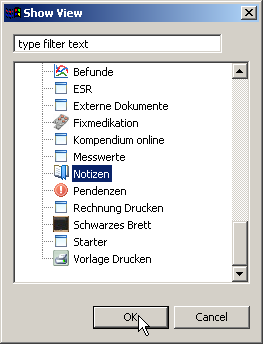
\includegraphics[width=3in]{images/notizen1}
% notizen1.png: 263x344 pixel, 96dpi, 6.96x9.10 cm, bb=0 0 197 258

Folgendes Fenster öffnet sich (bei Ihnen allerdings vermutlich noch ohne Inhalte):

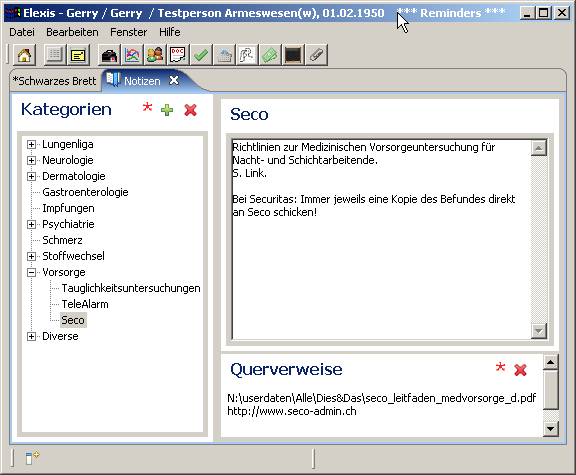
\includegraphics[width=3in]{images/notizen2}
% notizen2.png: 576x475 pixel, 96dpi, 15.24x12.57 cm, bb=0 0 432 356

Notizen können beliebig strukturiert und hierarchisch geordnet werden. Jede Notiz kann Text,
 Verweise auf externe Dokumente und Unterkategorien enthalten.

\begin{itemize}
 \item Um eine neue Hauptkategorie zu erstellen, klicken Sie auf das Stern-Symbol bei \textit{Kategorien}.
\item Um eine neue Unterkategorie zu erstellen, markieren Sie die Notiz, unter die diese Kategorie eingetragen werden soll, und klicken Sie auf das Plus-Symbol bei \textit{Kategorien}.
\item Um eine Notiz und alle ihr zugeordneten Unterkategorien zu löschen, klicken Sie auf das X - Symbol bei \textit{Kategorien}.
\item Um einen Text zu einer Kategorie oder einer Notiz zu erfassen, tippen Sie ihn einfach im rechten Fenster ein. Er wird automatisch sofort gespeichert. Sie können ihn jederzeit ändern.
\item Um einer Notiz oder einer Kategorie eine externe Datei oder eine Website zuzuordnen, klicken Sie auf das Stern-Symbol bei \textit{Querverweise}. Sie können dann den Pfad zu dieser Datei bzw. die URL der Website eingeben.
\item Um eine verknüpfte Datei anzusehen oder zu ändern, doppelklicken Sie auf den Querverweis.
\item Um eine Verknüpfung (aber nicht die Datei selbst!) zu löschen, klicken Sie auf das X-Symbol bei \textit{Querverweise}.
\end{itemize}

\subsection{Hinweise}

\begin{itemize}
 \item Notizen werden in der Datenbank gespeichert und sind grundsätzlich von allen angeschlossenen Arbeitsstationen und allen Anwendern lesbar.
\item Verknüpfte Dateien werden nur verknüpft, nicht in die Datenbank importiert. Sie können von anderen Arbeitsstationen aus nur dann geöffnet werden, wenn dort derselbe Pfad zur entsprechenden Datei gesetzt ist - in aller Regel wird dies ein gemeinsames Verzeichnis auf dem Server sein müssen.
\item Verknüpfte Dateien werden jeweils mit der im Betriebssystem für diesen Dateityp registrierten Anwendung geöffnet. Also beispielsweise Acrobat Reader für PDF-Dateien. Man kann solche Dateien deswegen nur von denjenigen Arbeitsstationen aus öffnen, die die entsprechende Anwendung installiert haben.
\end{itemize}

Um dieses Fenster dauerhaft in die gewählte Perspektive einzubinden, wählen
Sie \textit{Fenster-Speichere Perspektive}.

